\documentclass[11pt]{scrartcl}
\usepackage[usenames,dvipsnames,svgnames]{xcolor}
\usepackage[shortlabels]{enumitem}
\usepackage[framemethod=TikZ]{mdframed}
\usepackage{amsmath,amssymb,amsthm}
\usepackage{epigraph}
\usepackage[colorlinks]{hyperref}
\usepackage{microtype}
\usepackage{mathtools}
\usepackage[headsepline]{scrlayer-scrpage}
\usepackage{thmtools}
\usepackage{listings}
\usepackage{derivative}
\renewcommand{\epigraphsize}{\scriptsize}
\renewcommand{\epigraphwidth}{60ex}
\addtolength{\textheight}{3.14cm}
\ihead{\footnotesize\textbf{DGW-harmonic}}
\ohead{\footnotesize Updated Mon 8 Jan 2024 20:42:31 UTC}
\providecommand{\clubs}[1]{$#1\clubsuit$}
\providecommand{\clubg}[1]{\bgroup\color{green!40!black}[$#1\clubsuit$]\egroup}

\providecommand{\ol}{\overline}
\providecommand{\eps}{\varepsilon}
\providecommand{\half}{\frac{1}{2}}
\providecommand{\dang}{\measuredangle} %% Directed angle
\providecommand{\CC}{\mathbb C}
\providecommand{\FF}{\mathbb F}
\providecommand{\NN}{\mathbb N}
\providecommand{\QQ}{\mathbb Q}
\providecommand{\RR}{\mathbb R}
\providecommand{\ZZ}{\mathbb Z}
\providecommand{\dg}{^\circ}
\providecommand{\ii}{\item}
\providecommand{\alert}{\textbf}
\providecommand{\opname}{\operatorname}
\providecommand{\ts}{\textsuperscript}
% hacks for arc
\providecommand{\tarc}{\mbox{\large$\frown$}}
\providecommand{\arc}[1]{\stackrel{\tarc}{#1}}
\reversemarginpar
\providecommand{\printpuid}[1]{\marginpar{\href{https://otis.evanchen.cc/arch/#1}{\ttfamily\footnotesize\color{green!40!black}#1}}}

\mdfdefinestyle{mdbluebox}{roundcorner=10pt,innerbottommargin=9pt,
    linecolor=blue,backgroundcolor=TealBlue!5,}
\declaretheoremstyle[headfont=\sffamily\bfseries\color{MidnightBlue},
    mdframed={style=mdbluebox},]{thmbluebox}
\mdfdefinestyle{mdredbox}{frametitlefont=\bfseries,innerbottommargin=8pt,
    nobreak=true,backgroundcolor=Salmon!5,linecolor=RawSienna,}
\declaretheoremstyle[headfont=\bfseries\color{RawSienna},
    mdframed={style=mdredbox},headpunct={\\[3pt]},postheadspace=0pt,]{thmredbox}
\mdfdefinestyle{mdgreenbox}{linecolor=ForestGreen,backgroundcolor=ForestGreen!5,
    linewidth=2pt,rightline=false,leftline=true,topline=false,bottomline=false,}
\declaretheoremstyle[headfont=\bfseries\sffamily\color{ForestGreen!70!black},
    mdframed={style=mdgreenbox},headpunct={ --- },]{thmgreenbox}
\mdfdefinestyle{mdblackbox}{linecolor=black,backgroundcolor=RedViolet!5!gray!5,
    linewidth=3pt,rightline=false,leftline=true,topline=false,bottomline=false,}
\declaretheoremstyle[mdframed={style=mdblackbox}]{thmblackbox}
\declaretheorem[style=thmredbox,name=Problem]{problem}
\declaretheorem[style=thmredbox,name=Required Problem,sibling=problem]{reqproblem}
\declaretheorem[style=thmbluebox,name=Theorem,numberwithin=problem]{theorem}
\declaretheorem[style=thmbluebox,name=Lemma,sibling=theorem]{lemma}
\declaretheorem[style=thmbluebox,name=Theorem,numbered=no]{theorem*}
\declaretheorem[style=thmbluebox,name=Lemma,numbered=no]{lemma*}
\declaretheorem[style=thmgreenbox,name=Claim,sibling=theorem]{claim}
\declaretheorem[style=thmgreenbox,name=Claim,numbered=no]{claim*}
\declaretheorem[style=thmblackbox,name=Remark,sibling=theorem]{remark}
\declaretheorem[style=thmblackbox,name=Remark,numbered=no]{remark*}
\declaretheorem[style=thmgreenbox,name=Definition,sibling=theorem]{definition}
\declaretheorem[style=thmgreenbox,name=Definition,numbered=no]{definition*}
\declaretheorem[style=thmblackbox,name=Example,sibling=theorem]{example}
\declaretheorem[style=thmblackbox,name=Example,numbered=no]{example*}

\newenvironment{walkthrough}{\noindent\textbf{\color{green!40!black}Walkthrough.}}{}
\newlist{walk}{enumerate}{3}
\setlist[walk]{label=\bfseries (\alph*)}

\usepackage{asymptote}
\begin{asydef}
size(8cm); // set a reasonable default
usepackage("amsmath");
usepackage("amssymb");
settings.tex="pdflatex";
settings.outformat="pdf";
import geometry;
void filldraw(picture pic = currentpicture, conic g, pen fillpen=defaultpen, pen drawpen=defaultpen) { filldraw(pic, (path) g, fillpen, drawpen); }
void fill(picture pic = currentpicture, conic g, pen p=defaultpen) { filldraw(pic, (path) g, p); }
pair foot(pair P, pair A, pair B) { return foot(triangle(A,B,P).VC); }
pair centroid(pair A, pair B, pair C) { return (A+B+C)/3; }
\end{asydef}

\newcommand{\goals}[2]{\bgroup
\sffamily\small \emph{Instructions}: Solve \clubg{#1}.
If you have time, solve \clubg{#2}.\egroup\par}

%% 426c616e6b204c615465587e
\begin{document}
\title{Submission for DGW-HARMONIC}
\subtitle{OTIS (internal use)}
\author{Michael Middlezong}
\date{\today}
\maketitle

\begin{example*}[Lemma 4.26 from my book, added by Catherine Xu, $0\clubsuit$]
  Let $\triangle ABC$ be a triangle, and let the tangents to
  its circumcircle at $B$ and $C$ meet at point $X$.
  Let $M$ be the midpoint of $\ol{BC}$.
  Show that $AX$ is the $A$-symmedian of $\triangle ABC$,
  meaning that $\dang BAX = \dang MAC$.
\end{example*} \printpuid{EGIMO426}

\begin{walkthrough}
Let $D$ be the intersection of $BC$ and $AX$, and let the tangent
of the circumcircle of $\triangle ABC$ at $A$ intersect $BC$ at the point $Y$.
\begin{walk}
  \ii Show that $(BC;DY) = -1$.
  \ii Show that the reflection of line $\ol{AY}$
  across the $\angle A$-bisector is parallel to $\ol{BC}$.
  \ii Take the reflection lines $AB$, $AC$, $AD$, $AY$ in (a)
  across the $\angle A$-bisector; these four lines are still harmonic.
  Use (b) to deduce the problem statement.
\end{walk}
\end{walkthrough}
%% You're not expected to write up walkthroughs (unless you really want to).
%% The source is just for your reference.

\begin{example*}[\href{https://aops.com/community/p3543136}{IMO 2014/4}, $0\clubsuit$]
  Let $P$ and $Q$ be on segment $BC$ of an acute triangle $ABC$
  such that $\angle PAB=\angle BCA$ and $\angle CAQ=\angle ABC$.
  Let $M$ and $N$ be points on $\ol{AP}$ and $\ol{AQ}$,
  respectively, such that $P$ is the midpoint of $\ol{AM}$
  and $Q$ is the midpoint of $\ol{AN}$.
  Prove that $\ol{BM}$ and $\ol{CN}$ meet on the
  circumcircle of $\triangle ABC$.
\end{example*} \printpuid{14IMO4}

\begin{walkthrough}
We give a walkthrough for the harmonic bundles solution.

\begin{walk}
  \ii Show that the tangent to $B$
  is parallel to $\ol{APM}$.
  \ii Find a natural harmonic bundle using the answer to (a).
\end{walk}
Let $\ol{BM}$ intersect the circumcircle again at $X$.
\begin{walk}[resume]
  \ii Projecting the answer to (b) onto the circumcircle
  gives a harmonic quadrilateral. Which one?
  \ii Deduce that $\ol{CN}$ passes through $X$ as well.
\end{walk}
\end{walkthrough}
%% You're not expected to write up walkthroughs (unless you really want to).
%% The source is just for your reference.

\begin{example*}[\href{https://aops.com/community/p2477427}{Brazil 2011/5}, $0\clubsuit$]
  Let $ABC$ be an acute triangle
  with orthocenter $H$ and altitudes $\ol{BD}$, $\ol{CE}$.
  The circumcircle of $ADE$ cuts the circumcircle of $ABC$ at $F \neq A$.
  Prove that the angle bisectors of $\angle BFC$ and $\angle BHC$
  concur at a point on $\ol{BC}$.
\end{example*} \printpuid{11BRA5}

\begin{walkthrough}
There are two general approaches, one by harmonic
quadrilaterals and one by spiral similarity.
Both begin the same way.
\begin{walk}
  \ii Show that the condition is equivalent
  to $FB/FC = HB/HC$.
\end{walk}
\begin{center}
\begin{asy}
size(5cm);
pair A = dir(110);
pair B = dir(210);
pair C = dir(330);
pair H = orthocenter(A, B, C);
pair D = foot(B, A, C);
pair E = foot(C, A, B);
pair F = foot(H, A, extension(D, E, B, C));

draw(A--B--C--cycle, orange);
filldraw(circumcircle(A, B, C), opacity(0.1)+orange, orange);
filldraw(circumcircle(D, E, F), opacity(0.1)+red, yellow);
draw(B--D, orange);
draw(C--E, orange);
draw(B--F--C, orange);
pair L = extension(A, H, B, C);
draw(A--L, orange);

pair X = extension(A, H, -A, (B-C)-A);

dot("$A$", A, dir(A));
dot("$B$", B, dir(B));
dot("$C$", C, dir(C));
dot("$H$", H, dir(315));
dot("$D$", D, dir(D));
dot("$E$", E, dir(E));
dot("$F$", F, dir(F));
dot("$L$", L, dir(L));
\end{asy}
\end{center}
If you are working on the harmonic route:
\begin{walk}[resume]
  \ii Let $X$ be the intersection of ray $AH$
  with the circumcircle of $\triangle ABC$.
  Prove that the problem is equivalent to $FBXC$ being harmonic.
  \ii Show that lines $AF$, $DE$, $BC$ are concurrent.
  \ii Use (b) and (c) together to solve the problem.
\end{walk}
Here is a spiral similarity route:
\begin{walk}[resume]
  \ii Identify $F$ as a Miquel point of a quadrilateral,
  and write down the two pairs of similar triangles.
  \ii Use this to express $FB/FC$ as a ratio
  not involving the point $F$.
  \ii Show that the ratios you found in (f) are equal.
\end{walk}
Added bonus: the line $FH$ bisects $\ol{BC}$
and passes through the $A$-antipode.
\end{walkthrough}
%% You're not expected to write up walkthroughs (unless you really want to).
%% The source is just for your reference.

\begin{example*}[\href{https://aops.com/community/p1936916}{IMO 2010/4}, $0\clubsuit$]
  Let $P$ be a point interior to triangle $ABC$ (with $CA \neq CB$).
  The lines $AP$, $BP$ and $CP$ meet again its circumcircle $\Gamma$
  at $K$, $L$, $M$, respectively.
  The tangent line at $C$ to $\Gamma$ meets the line $AB$ at $S$.
  Show that from $SC = SP$ follows $MK = ML$.
\end{example*} \printpuid{10IMO4}

\begin{walkthrough}
Here is a walkthrough of a projective solution.

Let $D$ denote the other tangency point from $S$.
Let $\ol{DP}$ meet $(ABC)$ again at $N$.
\begin{walk}
  \ii Show that $KMLN$ is a harmonic quadrilateral.
  \ii We want to prove $MK = ML$.
  What does that suggest should be true about $MLNK$?
\end{walk}
In light of (b), our goal is to show that $\ol{MN}$ is a diameter.

It will make more sense actually to
let $N'$ be the antipode of $M$ on $\Gamma$,
and let $D'$ be the second intersection of $N'P$ with $\Gamma$.
We will show $D' = D$.
\begin{walk}[resume]
  \ii Show that $(CD'P)$ is orthogonal to $\Gamma$.
  (Possible hint: ``three tangents'' lemma in \S1 of EGMO.)
  \ii Identify the circumcenter of $\triangle CD'P$.
  \ii Show that $\ol{SD'}$ is tangent to $\Gamma$, so $D' = D$.
\end{walk}

So we now know have everything we need:
we know both that $\ol{MN}$ is a diameter and $\ol{SD}$ is tangent.
\begin{walk}[resume]
  \ii Deduce that $KLNM$ is a kite, and thus $NL = NK$.
\end{walk}
\end{walkthrough}
%% You're not expected to write up walkthroughs (unless you really want to).
%% The source is just for your reference.

\newpage

% ========================================
\section*{Practice problems}
\goals{45}{55}

\epigraph{Given three statements, two of them are equivalent.}
{Boris Alexeev, MOP 2003}

\begin{reqproblem}[Useful in later problems, $2\clubsuit$]
  Let $A$, $X$, $B$, $Y$ be points on a line in this order.
  Let $M$ be the midpoint of $\ol{AB}$.
  Show that the following are equivalent:
  \begin{itemize}
  \ii $(AB;XY) = -1$.
  \ii $MA^2 = MX \cdot MY$ and $AX > XB$.
  \ii $YA \cdot YB = YX \cdot YM$.
  \end{itemize}
  (Try to find ``synthetic'' solutions involving circles.
  This is a useful lemma in many problems, so keep it in mind!)
\end{reqproblem} \printpuid{Z79810E7}

%% Type your solution to Useful in later problems (\href{https://otis.evanchen.cc/arch/Z79810E7/}{Z79810E7}) here ...
Let $\omega$ be the circle with diameter $\ol{AB}$,
and let $\gamma$ be the circle with diameter $\ol{XY}$.

The first condition is equivalent to $X$ mapping to $Y$ under inversion around $\omega$.
This means the circles are orthogonal, and thus,
\[ MA^2 = MP^2 = MX \cdot MY. \]
Also, we have
\[ YA \cdot YB = YM^2 - MA^2 = YM^2 - XM \cdot YM = YM(YM - XM) = YM \cdot YX, \]
as desired.
%% --------------------------------------------------

\begin{problem}[EGMO Lemma 9.27: Self-Polar Orthogonality, $2\clubsuit$]
  Let $\omega$ be a circle and suppose $P$ and $Q$ are points
  such that $P$ lies on the polar of $Q$
  (and hence $Q$ lies on the polar of $P$).
  Prove that the circle $\gamma$
  with diameter $\ol{PQ}$ is orthogonal to $\omega$.
\end{problem} \printpuid{EGIMO927}

%% Type your solution to EGMO Lemma 9.27: Self-Polar Orthogonality (\href{https://otis.evanchen.cc/arch/EGIMO927/}{EGIMO927}) here ...
Let $D$ be the foot of the perpendicular from $P$ to line $OQ$.
Notice that since $\triangle DPQ$ is right, $D$ must lie on circle $\gamma$.
Moreover, an inversion around $\omega$ takes $D$ to $Q$, since $DP$ is the polar of $Q$.
Thus, $\gamma$ maps to itself under this inversion, so it is orthogonal to $\omega$.
%% --------------------------------------------------

\begin{problem}[\href{https://aops.com/community/p2268953}{Canada 1994}, $2\clubsuit$]
  Let $ABC$ be an acute triangle.
  Let $\ol{AD}$ be the altitude on $\ol{BC}$,
  and let $H$ be any interior point on $\ol{AD}$.
  Lines $BH$ and $CH$, when extended,
  intersect $\ol{AC}$, $\ol{AB}$ at $E$ and $F$ respectively.

  Prove that $\angle EDH=\angle FDH$.
\end{problem} \printpuid{94CAN5}

%% Type your solution to Canada 1994 (\href{https://otis.evanchen.cc/arch/94CAN5/}{94CAN5}) here ...
Intersect line $EF$ with line $BC$, and the problem becomes trivial
using the right angles and bisectors lemma.
%% --------------------------------------------------

\begin{problem}[\href{https://aops.com/community/p26404400}{PAGMO 2022/3}, $2\clubsuit$]
  Let $ABC$ be an acute triangle with $AB< AC$.
  Denote by $P$ and $Q$ points on the segment $BC$
  such that $\angle BAP = \angle CAQ < \frac{\angle BAC}{2}$.
  Point $B_1$ lies on segment $AC$,
  and $BB_1$ intersects $AP$ and $AQ$ at $P_1$ and $Q_1$, respectively.
  The angle bisectors of $\angle BAC$ and $\angle CBB_1$ intersect at $M$.
  If $PQ_1\perp AC$ and $QP_1\perp AB$, prove that $AQ_1MPB$ is cyclic.
\end{problem} \printpuid{22PAGMO3}

%% Type your solution to PAGMO 2022/3 (\href{https://otis.evanchen.cc/arch/22PAGMO3/}{22PAGMO3}) here ...

%% --------------------------------------------------

\begin{reqproblem}[\href{https://aops.com/community/p2728462}{ELMO SL 2012 G3}, $3\clubsuit$]
  Let $ABC$ be a triangle with incenter $I$.
  The foot of the perpendicular from $I$ to $\ol{BC}$ is $D$,
  and the foot of the perpendicular from $I$ to $\ol{AD}$ is $P$.
  Prove that $\angle BPD = \angle DPC$.
\end{reqproblem} \printpuid{12ESLG3}

%% Type your solution to ELMO SL 2012 G3 (\href{https://otis.evanchen.cc/arch/12ESLG3/}{12ESLG3}), proposed by Alex Zhu here ...
If $AB = AC$, then we are done by symmetry. Otherwise, let $K$ be the intersection point of lines $IP$ and $BC$.
Notice that $K$ is the inverse of $P$ with respect to the incircle, and thus, $A$ lies on the polar of $K$.
By La Hire's theorem, we know that $K$ lies on the polar of $A$. In other words, if $E$ and $F$ are the contact
points of the incircle with sides $AC$ and $AB$, respectively, then $K$ lies on line $EF$.

It is well known that the cevians $AD$, $BE$, and $CF$ concur, so we can use the concurrent cevians lemma to deduce
that $(ED;BC) = -1$. Finally, since $\angle EPD = 90$, the right angles and bisectors lemma tells us that
$\angle BPD = \angle DPC$.
%% --------------------------------------------------

\begin{problem}[\href{https://aops.com/community/p2254813}{JMO 2011/5}, $2\clubsuit$]
  Points $A,B,C,D,E$ lie on a circle $\omega$
  and point $P$ lies outside the circle.
  The given points are such that
  (i) lines $PB$ and $PD$ are tangent to $\omega$,
  (ii) $P, A, C$ are collinear,
  and (iii) $\ol{DE} \parallel \ol{AC}$.
  Prove that $\ol{BE}$ bisects $\ol{AC}$.
\end{problem} \printpuid{11JMO5}

%% Type your solution to JMO 2011/5 (\href{https://otis.evanchen.cc/arch/11JMO5/}{11JMO5}), proposed by Zuming Feng here ...
Letting $M = \ol{BE} \cap \ol{AC}$ and $F$ be the second intersection point of line $DM$ with $\omega$,
we have
\[ -1 = (CA;DB) \overset M= (AC;FE) \overset D= (AC;M\infty), \]
and thus, $M$ is the midpoint of $AC$.
%% --------------------------------------------------

\begin{problem}[MOP 2013, $2\clubsuit$]
  Let $ABC$ be an acute scalene triangle,
  and let $H$ be a point inside it such that $\ol{AH} \perp \ol{BC}$.
  Rays $BH$ and $CH$ meet $\ol{AC}$ and $\ol{AB}$ at $E$, $F$.
  Prove that if quadrilateral $BFEC$ is cyclic
  then $H$ is in fact the orthocenter of $ABC$.
\end{problem} \printpuid{13MOPHWR8}

%% Type your solution to MOP 2013 (\href{https://otis.evanchen.cc/arch/13MOPHWR8/}{13MOPHWR8}) here ...
Let $X$ be the intersection point of line $EF$ with line $BC$.
Let $M$ be the center of $(BFEC)$.
Brocard's theorem tells us that $M$ is the orthocenter of triangle $AXH$.
This means that $\ol{XM} \perp \ol{AD}$, and thus, $M$ must be the midpoint of $BC$.
The desired result easily follows from here.
%% --------------------------------------------------

\begin{problem}[\href{https://aops.com/community/p23322980}{PAGMO 2021/6}, $3\clubsuit$]
  Let $ABC$ be a triangle with incenter $I$, and $A$-excircle $\Gamma$.
  Let $A_1$, $B_1$, $C_1$ be the points of tangency of $\Gamma$
  with $BC$, $AC$ and $AB$, respectively.
  Suppose $IA_1$, $IB_1$ and $IC_1$ intersect $\Gamma$ for the second time
  at points $A_2$, $B_2$, $C_2$, respectively.
  $M$ is the midpoint of segment $AA_1$.
  If the intersection of $A_1B_1$ and $A_2B_2$ is $X$,
  and the intersection of $A_1C_1$ and $A_2C_2$ is $Y$, prove that $MX=MY$.
\end{problem} \printpuid{21PAGMO6}

%% Type your solution to PAGMO 2021/6 (\href{https://otis.evanchen.cc/arch/21PAGMO6/}{21PAGMO6}) here ...

%% --------------------------------------------------

\begin{reqproblem}[\href{https://aops.com/community/p12623614}{ELMO Shortlist 2019 G1, added by Kevin Wang}, $5\clubsuit$]
  Let $ABC$ be an acute triangle with orthocenter $H$
  and circumcircle $\Gamma$.
  Let $BH$ intersect $AC$ at $E$, and let $CH$ intersect $AB$ at $F$.
  Let $AH$ intersect $\Gamma$ again at $P \neq A$.
  Let $PE$ intersect $\Gamma$ again at $Q \neq P$.
  Prove that $BQ$ bisects segment $\ol{EF}$.
\end{reqproblem} \printpuid{19ESLG1}

%% Type your solution to ELMO Shortlist 2019 G1, added by Kevin Wang (\href{https://otis.evanchen.cc/arch/19ESLG1/}{19ESLG1}), proposed by Luke Robitaille here ...
Let $D$ be the foot of the altitude from $A$ to $BC$,
let $M = \ol{BQ} \cap \ol{EF}$,
let $S$ be the second intersection of $(AEF)$ with $\Gamma$,
let $X = \ol{EF} \cap \ol{BC}$,
let $R$ be the second intersection of line $BE$ and $\Gamma$,
and let $K$ be the point on $\Gamma$ satisfying $\ol{BK} \parallel \ol{EF}$.
\begin{center}
    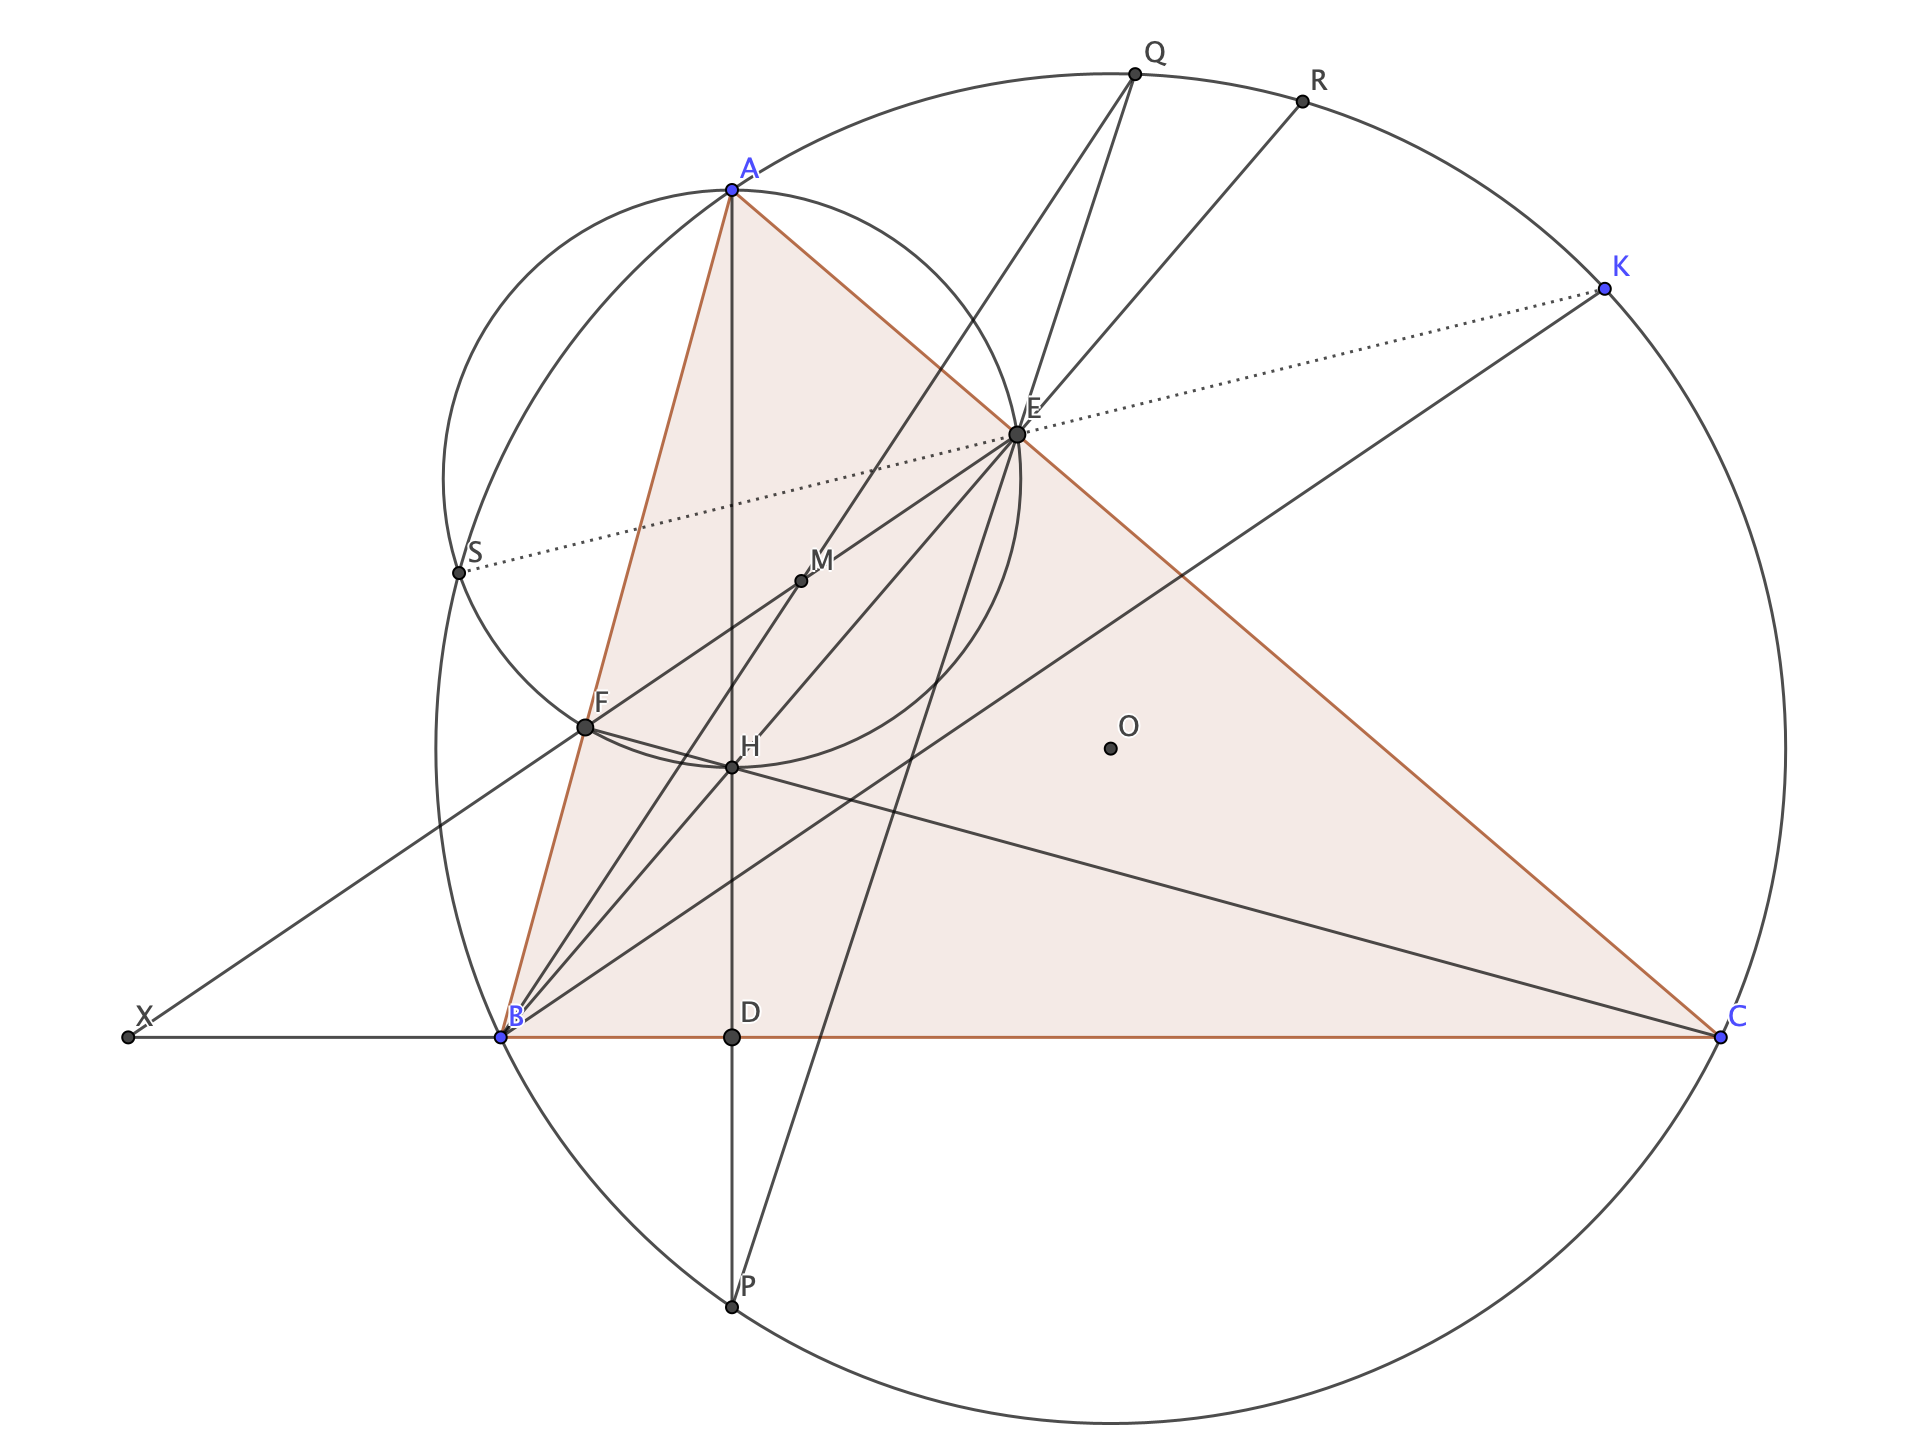
\includegraphics[width=10cm]{19ESLG1.png}
\end{center}

First, we show $S$, $E$, $K$ are collinear. This is trivial by angle chasing:
\[ \angle ASE = \angle AFE = \angle ABK = \angle ASK. \]
Now, notice that $A$, $S$, and $X$ are collinear. This is well known and the proof is by radical axis.
Finally,
\[ -1 = (XD;BC) \overset A= (SP;BC) \overset E= (KQ;RA) \overset B= (\infty M;EF), \]
and we are done.
%% --------------------------------------------------

\begin{problem}[\href{https://aops.com/community/p3551910}{Taiwan TST 2014/1J/3}, $3\clubsuit$]
  In $\triangle ABC$ with incenter $I$,
  the incircle is tangent to $\ol{CA}$, $\ol{AB}$ at $E$, $F$.
  The reflections of $E$, $F$ across $I$ are $G$, $H$.
  Let $Q$ be the intersection of $\ol{GH}$ and $\ol{BC}$,
  and let $M$ be the midpoint of $\ol{BC}$.
  Prove that $\ol{IQ}$ and $\ol{IM}$ are perpendicular.
\end{problem} \printpuid{14TWNTST1J3}

%% Type your solution to Taiwan TST 2014/1J/3 (\href{https://otis.evanchen.cc/arch/14TWNTST1J3/}{14TWNTST1J3}) here ...
Let $D$ be the contact point of the incircle with $BC$,
let $Q'$ be the intersection of lines $QI$ and $EF$,
and let $D'$ be the antipode of $D$.
\begin{center}
    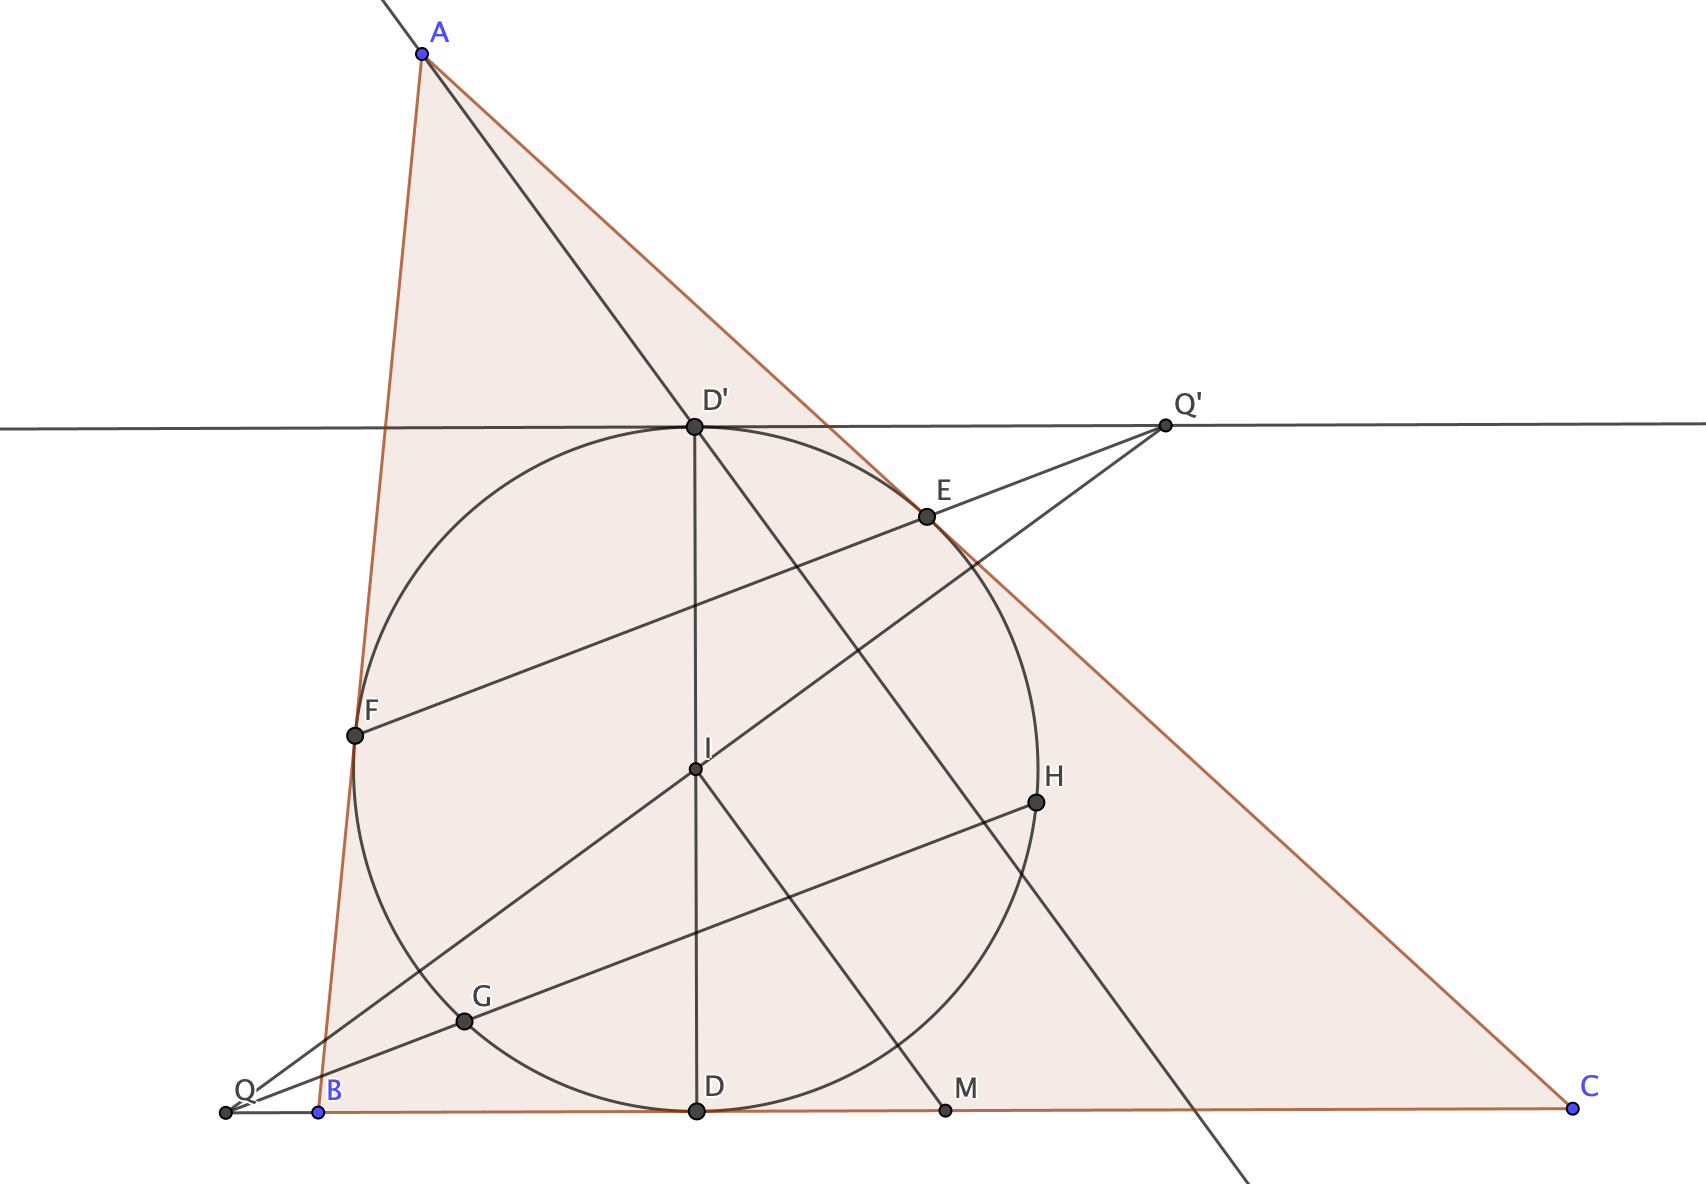
\includegraphics[width=10cm]{14TWNTST1J3.png}
\end{center}

By symmetry, $\ol{Q'D'} \parallel \ol{BC}$, and thus,
$\ol{Q'D'}$ is tangent to the incircle.
Then, by La Hire's theorem, $Q'$ is the pole of line $AD'$.
Finish by noticing that $\ol{AD} \parallel \ol{IM}$ (well-known; proof is by homothety).
%% --------------------------------------------------

\begin{reqproblem}[Sloth blocking ruler, $3\clubsuit$]
  You have a large sheet of paper in which
  three marked points $A$, $B$, $C$ are collinear in that order.
  You want to construct line $ABC$ with your straightedge,
  but a cute sloth is sleeping peacefully on the paper
  and obstructing the segment $BC$.
  Determine how to extend ray $AB$ past $C$
  without disturbing the sloth (with straightedge alone).
\end{reqproblem} \printpuid{Z8AF8A34}

%% Type your solution to Sloth blocking ruler (\href{https://otis.evanchen.cc/arch/Z8AF8A34/}{Z8AF8A34}) here ...
First, if $AB \le BC$, we can extend ray $BA$ and move point $A$ so that $AB > BC$.

Draw point $D$ not on line $ABC$.
Draw lines $DA$, $DB$, and $DC$.
Pick a point $P$ on $DB$.
Now, we create the Ceva/Menelaus configuration as follows:

Extend ray $AP$ to hit $DC$ at $E$ and ray $CP$ to hit $DA$ at $F$.
Notice that the intersection point with line $EF$ and line $AC$, which we want,
is just the harmonic conjugate of $\ol{DB} \cap \ol{EF}$ with respect to $EF$.
However, this line is actaully accessible to us, so we can just
repeat this configuration again to obtain the desired point.
%% --------------------------------------------------

\begin{problem}[\href{https://aops.com/community/c6h2619p3309010}{Iran 2002}, $5\clubsuit$]
  Let $ABC$ be a triangle. The incircle of triangle $ABC$ touches the side $BC$ at $A'$, and the line $AA'$ meets the incircle again at a point $P$. Let the lines $CP$ and $BP$ meet the incircle of triangle $ABC$ again at $N$ and $M$, respectively. Prove that the lines $AA'$, $BN$ and $CM$ are concurrent.
\end{problem} \printpuid{02IRN}

%% Type your solution to Iran 2002 (\href{https://otis.evanchen.cc/arch/02IRN/}{02IRN}) here ...
\begin{center}
    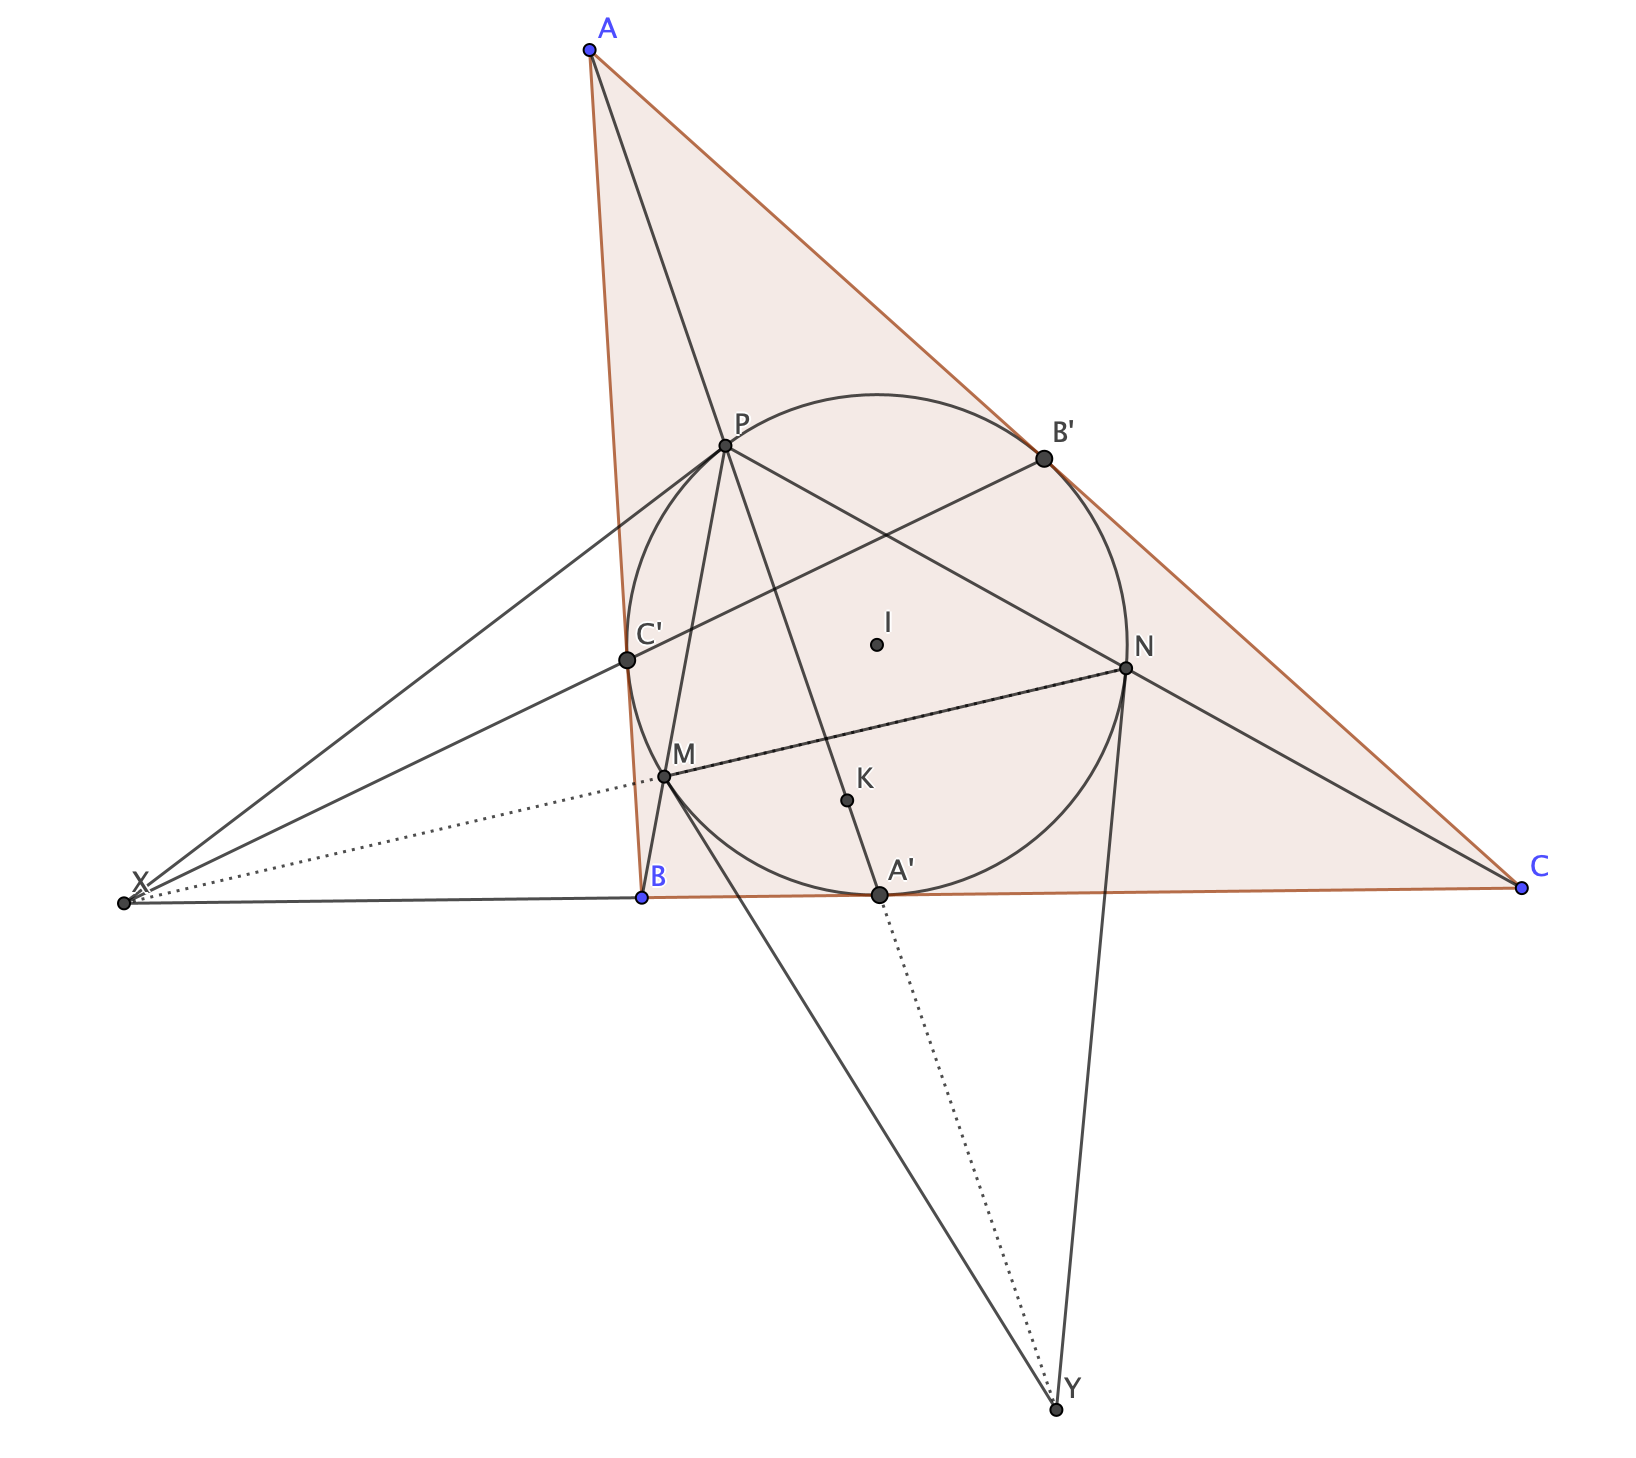
\includegraphics[width=10cm]{02IRN.png}
\end{center}
Let $B'$ and $C'$ be the other two incircle contact points,
and let $X$ be the intersection point of line $B'C'$ and line $BC$.
It is well known that $X$ is the pole of line $PA'$, and thus,
line $XP$ is tangent to the incircle.

Notice that by the Ceva/Menelaus configuration, the problem is equivalent
to showing that $X$, $M$, and $N$ are collinear.
Let $Y$ be the intersection point of the tangents to the incircle at $M$ and $N$.
By La Hire's theorem, it suffices to prove that $P$, $A'$, and $Y$ are collinear.
We have
\[ -1 = (XA';BC) \overset P= (PA';MN), \]
so by the symmedian config, line $PY$ intersects the incircle at $A'$, so we are done.
%% --------------------------------------------------

\begin{problem}[Kazakhstan 2011/9.5, $3\clubsuit$]
  Given a non-degenerate triangle $ABC$,
  let $A_1$, $B_1$, $C_1$ be the points of tangency
  of the incircle to the sides $BC$, $CA$, $AB$.
  Let $Q$ and $L$ be the intersection of the segment $AA_{1}$
  with the incircle and the segment $B_{1}C_{1}$ respectively.
  Let $M$ be the midpoint of $B_{1}C_{1}$.
  Let $T$ be the point of intersection of $BC$ and $B_{1}C_{1}$.
  Let $P$ be the foot of the perpendicular from the
  point $L$ on the line $AT$.
  Prove that the points $A_1, M, Q, P$ lie on a circle.
\end{problem} \printpuid{11KAZ95}

%% Type your solution to Kazakhstan 2011/9.5 (\href{https://otis.evanchen.cc/arch/11KAZ95/}{11KAZ95}) here ...

%% --------------------------------------------------

\begin{problem}[\href{https://aops.com/community/p5017915}{TSTST 2015/2}, $5\clubsuit$]
  Let $ABC$ be a scalene triangle. Let $K_a$, $L_a$, and
  $M_a$ be the respective intersections with $BC$ of the internal
  angle bisector, external angle bisector, and the median from
  $A$. The circumcircle of $AK_aL_a$ intersects $AM_a$ a second time
  at a point $X_a$ different from $A$. Define $X_b$ and $X_c$
  analogously. Prove that the circumcenter of $X_aX_bX_c$ lies on
  the Euler line of $ABC$.
\end{problem} \printpuid{15TSTST2}

%% Type your solution to TSTST 2015/2 (\href{https://otis.evanchen.cc/arch/15TSTST2/}{15TSTST2}), proposed by Ivan Borsenco here ...

%% --------------------------------------------------

\begin{problem}[\href{https://aops.com/community/p10632290}{Shortlist 2017 G4}, $5\clubsuit$]
  Let $ABC$ be a triangle and let $\omega$ be the $A$-excircle,
  tangent to $\ol{BC}$, $\ol{CA}$, $\ol{AB}$ at $D$, $E$, $F$.
  The circumcircle of $\triangle AEF$ intersects line $BC$ at $P$ and $Q$.
  Let $M$ be the midpoint of $\ol{AD}$.
  Prove that the circumcircle of $\triangle MPQ$ is tangent to $\omega$.
\end{problem} \printpuid{17SLG4}

%% Type your solution to Shortlist 2017 G4 (\href{https://otis.evanchen.cc/arch/17SLG4/}{17SLG4}) here ...
Let $W$ be the center of $\omega$,
let $K$ be the intersection of lines $EF$ and $BC$,
and let $T$ be the second intersection of line $AD$ with $\omega$.
We claim that $T$ is the desired point of tangency.
\begin{center}
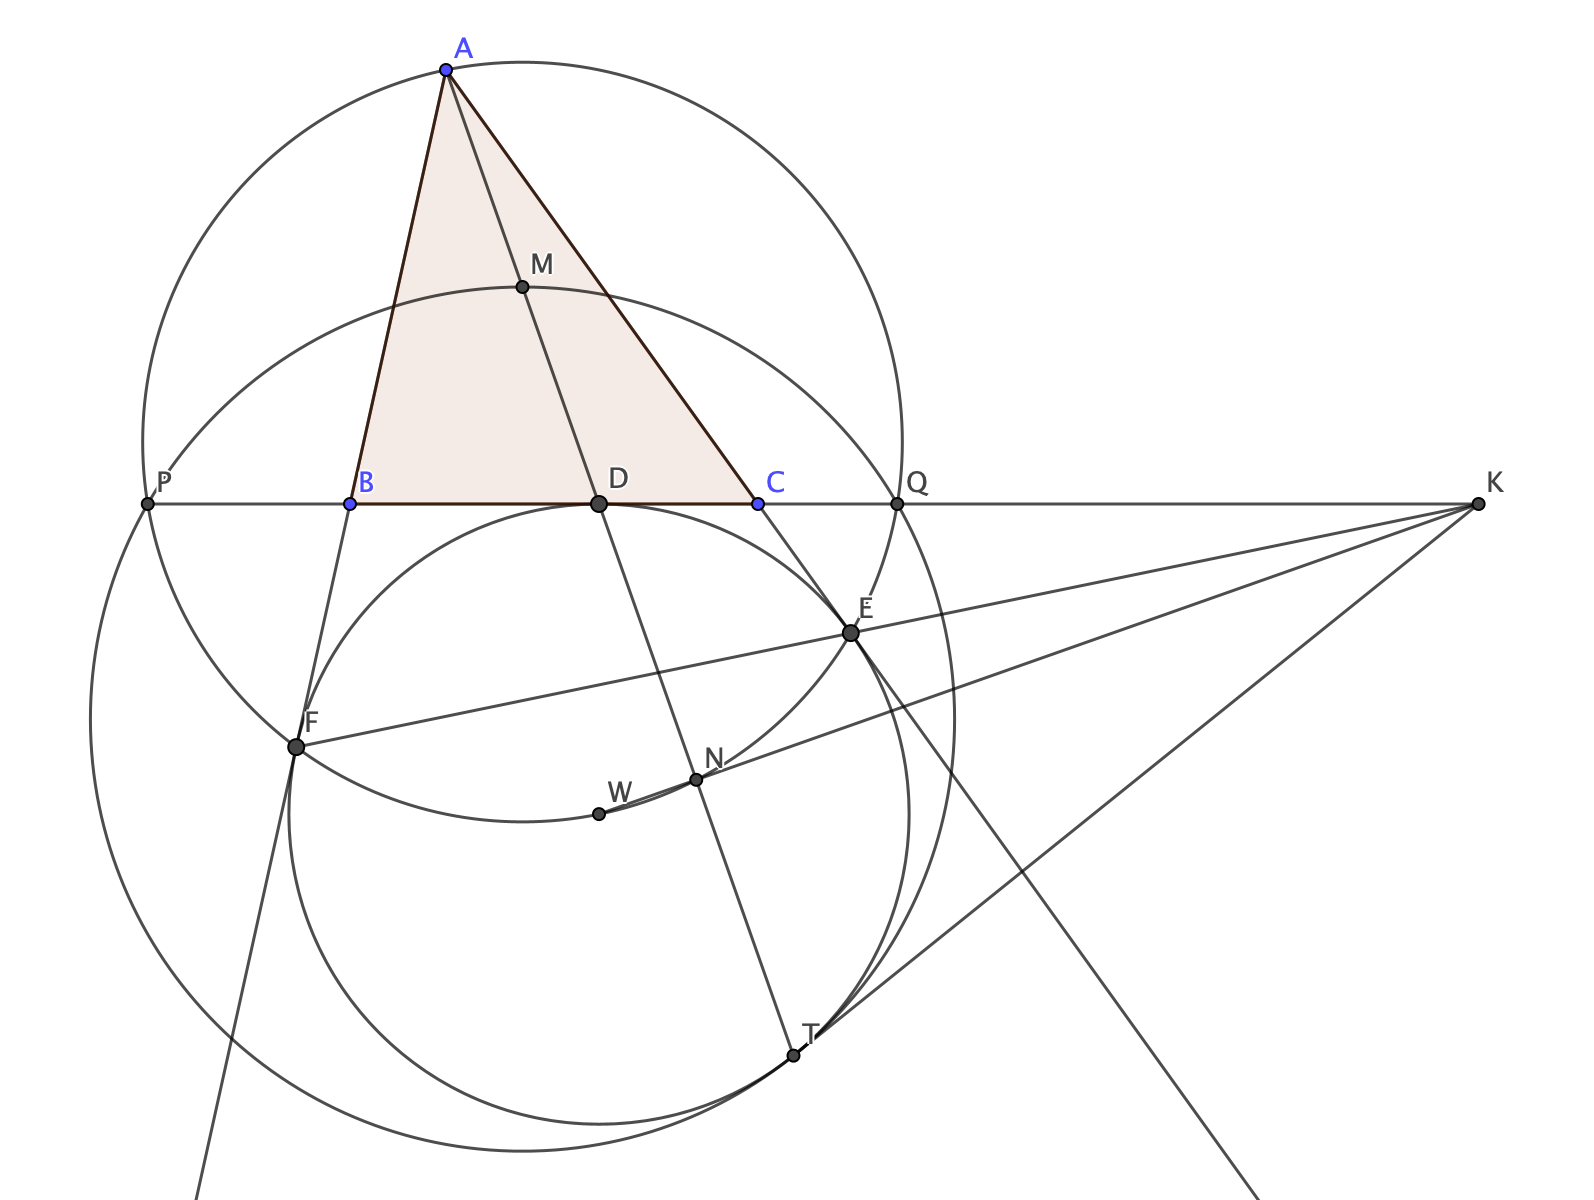
\includegraphics[width=10cm]{17SLG4.png}
\end{center}

First, notice that $FDET$ is harmonic, so line $KT$ is tangent to $\omega$.

Let $N$ be the midpoint of $DT$.
Notice that $W$ lies on $(AEF)$ by angle chasing,
and $N$ lies on $(AEF)$ because $WN \perp AN$.

Also, $T$ lies on $(MPQ)$ because $DT \cdot DM = DN \cdot DA = DP \cdot DQ$.

Finally, we have
\[ KP \cdot KQ = KF \cdot KE = KT^2, \]
so by power of a point, we are done.
%% --------------------------------------------------

\begin{problem}[\href{https://aops.com/community/p13155392}{Iran Geo Olympiad 2019, added by Tilek Askerbekov}, $3\clubsuit$]
  Circles $\omega_1$ and $\omega_2$ have centers $O_1$ and $O_2$, respectively.
  These two circles intersect at points $X$ and $Y$.
  Line $AB$ is a common tangent of these two circles
  such that $A$ lies on $\omega_1$ and $B$ lies on $\omega_2$.
  Let the tangents to $\omega_1$ and $\omega_2$ at $X$ intersect $O_1O_2$
  at points $K$ and $L$, respectively.
  Suppose that line $BL$ intersects $\omega_2$ again at $M$
  and $AK$ intersects $\omega_1$ again at $N$.
  Prove that $AM$, $BN$ and $O_1O_2$ concur.
\end{problem} \printpuid{19IGOA3}

%% Type your solution to Iran Geo Olympiad 2019, added by Tilek Askerbekov (\href{https://otis.evanchen.cc/arch/19IGOA3/}{19IGOA3}) here ...

%% --------------------------------------------------

\begin{problem}[\href{https://aops.com/community/p10148654}{Sharygin 2018, added by Kevin Wang}, $3\clubsuit$]
  Let scalene triangle $ABC$ have intouch triangle $XYZ$.
  The $A$-excircle touches the side $BC$ at point $N$.
  Let $T$ be the common point of $AN$ and the incircle,
  closest to $N$, and $K = \ol{YZ} \cap \ol{XT}$.
  Prove that $\ol{AK} \parallel \ol{BC}$.
\end{problem} \printpuid{18SHRG20}

%% Type your solution to Sharygin 2018, added by Kevin Wang (\href{https://otis.evanchen.cc/arch/18SHRG20/}{18SHRG20}) here ...

%% --------------------------------------------------

\begin{problem}[\href{https://aops.com/community/q1h481354p2696468}{South Africa 2005/4}, $2\clubsuit$]
  The inscribed circle of triangle $ABC$ touches the sides $BC$, $CA$ and $AB$ at $D$, $E$ and $F$ respectively. Let $Q$ denote the other point of intersection of $AD$ and the inscribed circle. Prove that $EQ$ extended passes through the midpoint of $AF$ if and only if $AC = BC$.
\end{problem} \printpuid{05SAF4}

%% Type your solution to South Africa 2005/4 (\href{https://otis.evanchen.cc/arch/05SAF4/}{05SAF4}) here ...
\begin{center}
    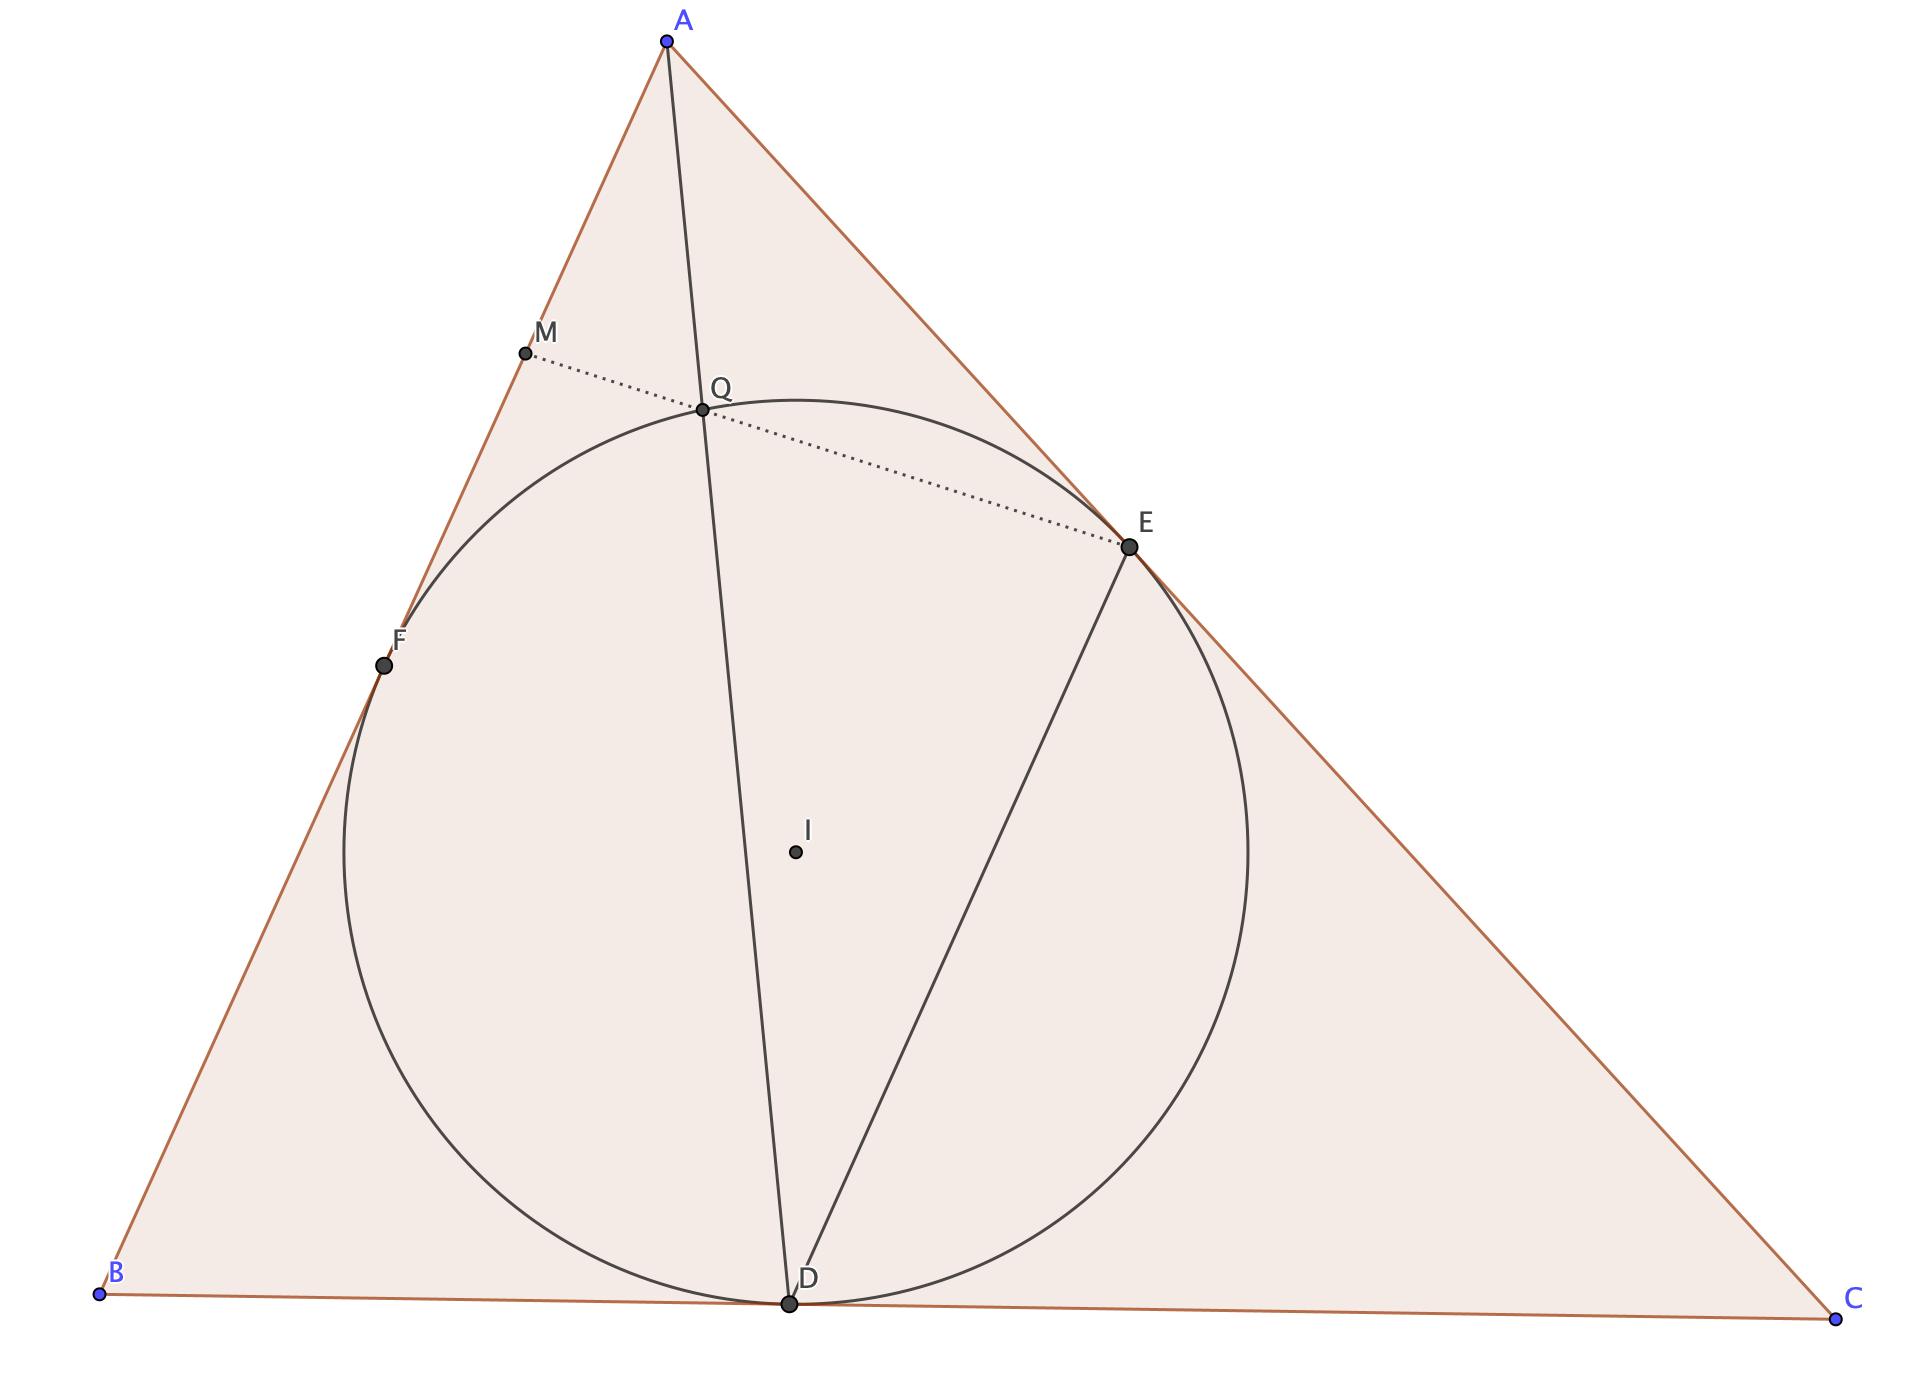
\includegraphics[width=8cm]{05SAF4.png}
\end{center}
Note that $(EF;DQ)=-1$. The problem is finished by considering the projection at $E$ onto line $AB$.
%% --------------------------------------------------

\begin{problem}[\href{https://aops.com/community/p463068}{Shortlist 2005 G6}, $5\clubsuit$]
  Let $ABC$ be a triangle, and $M$ the midpoint of its side $BC$.
  Let $\gamma$ be the incircle of triangle $ABC$.
  The median $AM$ of triangle $ABC$ intersects
  the incircle $\gamma$ at two points $K$ and $L$.
  Let the lines passing through $K$ and $L$,
  parallel to $\ol{BC}$,
  intersect the incircle $\gamma$ again in two points $X$ and $Y$.
  Let the lines $AX$ and $AY$ intersect $BC$ again at the points $P$ and $Q$.
  Prove that $BP = CQ$.
\end{problem} \printpuid{05SLG6}

%% Type your solution to Shortlist 2005 G6 (\href{https://otis.evanchen.cc/arch/05SLG6/}{05SLG6}) here ...

%% --------------------------------------------------

\begin{problem}[\href{https://aops.com/community/p10733925}{China Southeast MO 2018}, $5\clubsuit$]
  Let $ABC$ be an isosceles triangle with $AB = AC$.
  A circle $\Gamma$ centered at the midpoint $M$ of $\ol{BC}$
  is tangent to lines $AB$ and $AC$ at $F$ and $E$, respectively.
  Point $G$ is chosen on $\Gamma$ with $\angle AGE = 90\dg$.
  The tangents to $\Gamma$ at $G$ and $F$ meet at $K$.
  Prove that $\ol{CK}$ bisects $\ol{EF}$.
\end{problem} \printpuid{18CSMO6}

%% Type your solution to China Southeast MO 2018 (\href{https://otis.evanchen.cc/arch/18CSMO6/}{18CSMO6}) here ...

%% --------------------------------------------------

\begin{problem}[Added by William Zhao, $3\clubsuit$]
  Let $ABC$ be a right triangle with $\angle A = 90^\circ$,
  and let $D$ be a point lying on the side $AC$.
  Denote by $E$ reflection of $A$ into the line $BD$,
  and by $F$ the intersection point of $CE$ with the perpendicular in $D$ to the line $BC$.
  Prove that $AF$, $DE$ and $BC$ are concurrent.
\end{problem} \printpuid{ZD5935DF}

%% Type your solution to Added by William Zhao (\href{https://otis.evanchen.cc/arch/ZD5935DF/}{ZD5935DF}) here ...

%% --------------------------------------------------

\begin{problem}[\href{https://aops.com/community/h2648084}{Added by Krishna Pothapragada}, $3\clubsuit$]
  In $\triangle ABC$ with incenter $I$ and $A$-excenter $I_A$,
  let $G$ be the centroid of $\triangle BIC$.
  Define $E = \ol{BI} \cap \ol{AC}$ and $F = \ol{CI} \cap \ol{AB}$.
  Prove that $\angle BGC + \angle EI_AF = 180\dg$.
\end{problem} \printpuid{H2648084}

%% Type your solution to Added by Krishna Pothapragada (\href{https://otis.evanchen.cc/arch/H2648084/}{H2648084}) here ...

%% --------------------------------------------------

\begin{problem}[\href{https://aops.com/community/p7732197}{USA TST 2017, Danielle Wang}, $9\clubsuit$]
  Let $ABC$ be a triangle with altitude $\ol{AE}$.
  The $A$-excircle touches $\ol{BC}$ at $D$,
  and intersects the circumcircle at two points $F$ and $G$.
  Prove that one can select points $V$ and $N$
  on lines $DG$ and $DF$ such that quadrilateral $EVAN$ is a rhombus.
\end{problem} \printpuid{17USATST5}

%% Type your solution to USA TST 2017, Danielle Wang (\href{https://otis.evanchen.cc/arch/17USATST5/}{17USATST5}), proposed by Danielle Wang, Evan Chen here ...

%% --------------------------------------------------

\begin{problem}[\href{https://aops.com/community/p9853223}{HMMT 2018, added by Ram Goel}, $5\clubsuit$]
  Let $ABC$ be an equilateral triangle with side length $8$.
  Let $X$ be on side $AB$ so that $AX=5$ and $Y$ be on side $AC$ so that $AY=3$.
  Let $Z$ be on side $BC$ so that $AZ$, $BY$, $CX$ are concurrent.
  Let $ZX$, $ZY$ intersect the circumcircle of $AXY$ again at $P$, $Q$ respectively.
  Let $XQ$ and $YP$ intersect at $K$.
  Show that $KX\cdot KQ$ is an integer and determine its value.
\end{problem} \printpuid{18HMMTG8}

%% Type your solution to HMMT 2018, added by Ram Goel (\href{https://otis.evanchen.cc/arch/18HMMTG8/}{18HMMTG8}) here ...

%% --------------------------------------------------

\begin{reqproblem}[\href{https://aops.com/community/p5087419}{Taiwan TST Quiz 2015, by me}, $9\clubsuit$]
  In scalene triangle $ABC$ with incenter $I$, the incircle is tangent to
  sides $CA$ and $AB$ at points $E$ and $F$.
  The tangents to the circumcircle of $\triangle AEF$ at $E$ and $F$ meet at $S$.
  Lines $EF$ and $BC$ intersect at $T$.
  Prove that the circle with diameter $\ol{ST}$ is orthogonal to
  the nine-point circle of triangle $BIC$.
\end{reqproblem} \printpuid{15TWNQ3J6}

%% Type your solution to Taiwan TST Quiz 2015, by me (\href{https://otis.evanchen.cc/arch/15TWNQ3J6/}{15TWNQ3J6}), proposed by Evan Chen here ...
By the self-polar orthogonality lemma, it suffices to show that
$S$ lies on the polar of $T$ with respect to the nine-point circle.
\begin{center}
    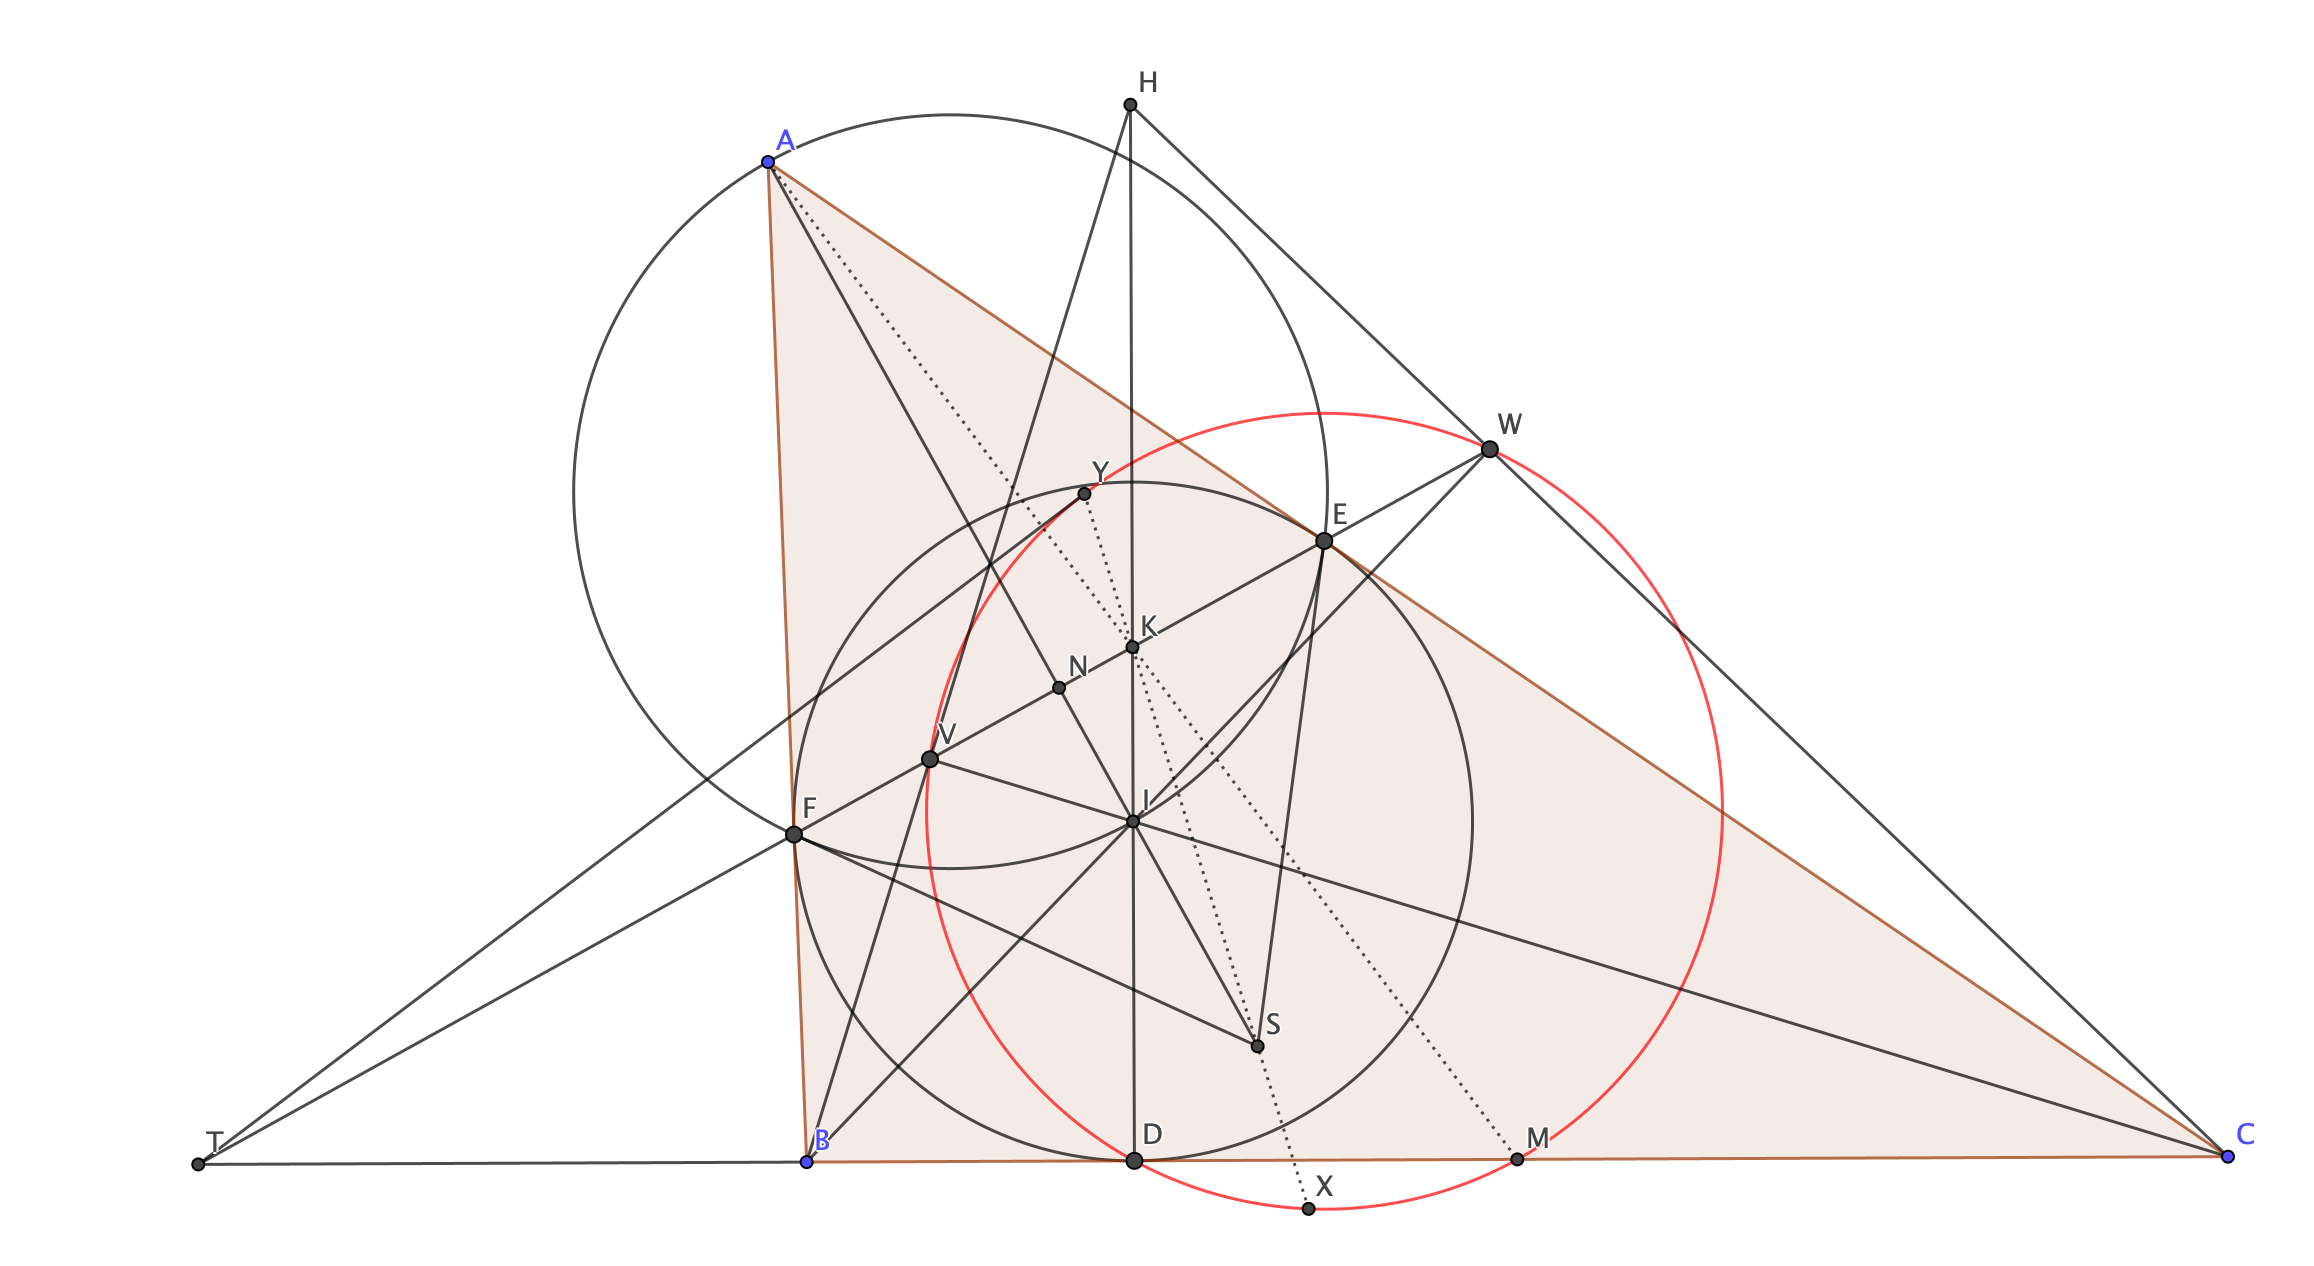
\includegraphics[width=10cm]{15TWNQ3J6.png}
\end{center}

To complete the nine-point circle configuration,
let $H$ be the orthocenter of $\triangle BIC$,
let $D$ be the remaining intouch point,
and let $M$ be the midpoint of $BC$.
Note that $D$ and $M$ lie on the nine-point circle,
and $I$ is the orthocenter of $\triangle HBC$.

Let $V$ and $W$ be the feet of the perpendiculars from $C$ and $B$
to their respective sides.
By the Iran lemma (proof: angle chasing), $V$ and $W$ lie on line $EF$.
Also, $V$ and $W$ lie on the nine-point circle.

Now, let $K$ be the intersection of lines $ID$ and $EF$,
let $N$ be the midpoint of $EF$,
and let $X$ and $Y$ be the points of tangency of $T$ with the nine-point circle.
We want to show that $X$, $Y$, and $S$ are collinear.

First, we have
\[ -1 = (TD;BC) \overset I= (TK;WV), \]
so $K$ lies on line $XY$.
Also, $K$ lies on line $AM$ by an incircle concurrency lemma.
So then,
\[ -1 = (AI;NS) \overset K= (M,D;T,\ol{KS}\cap\ol{BC}), \]
which means $\ol{KS}\cap\ol{BC}$ is on the polar of $T$.
Thus, $S$ is collinear with two points on the polar of $T$,
so $S$ must be on the polar of $T$, and we are done.
%% --------------------------------------------------

\end{document}
